\usetikzlibrary{arrows.meta, angles, quotes}

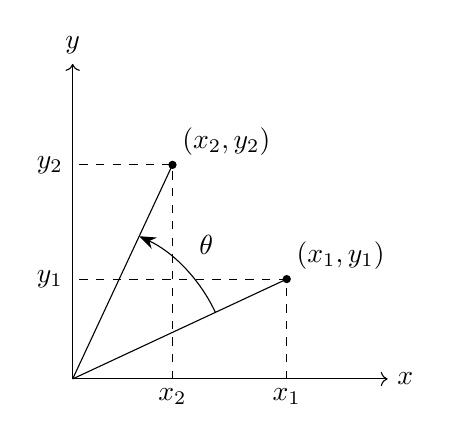
\begin{tikzpicture}
    % variables
    \pgfmathsetmacro{\vRadius}{3}
    \pgfmathsetmacro{\vPhi}{25}
    \pgfmathsetmacro{\vTheta}{40}

    \draw[->] (0,0) -- (4,0) node[right] {$x$};
    \draw[->] (0,0) -- (0,4) node[above] {$y$};

    \coordinate (O) at (0,0);
    \coordinate (A) at ({\vRadius*cos(\vPhi)},{\vRadius*sin(\vPhi)});
    \coordinate (B) at ({\vRadius*cos(\vPhi+\vTheta)},{\vRadius*sin(\vPhi+\vTheta)});

    \fill (A) circle (1.5pt);
    \fill (B) circle (1.5pt);

    \draw[-] (O) -- (A) node[above right] {$(x_1,y_1)$};
    \draw[-] (O) -- (B) node[above right] {$(x_2,y_2)$};

    \draw[dashed] (A |- O) node[below] {$x_1$} -- (A) -- (A -| O) node[left] {$y_1$};
    \draw[dashed] (B |- O) node[below] {$x_2$} -- (B) -- (B -| O) node[left] {$y_2$};

    \pic [draw,{-{Stealth[length=6pt]}},"$\theta$",angle radius=2cm,angle eccentricity=1.2] {angle=A--O--B};
\end{tikzpicture}